

\tikzset{every picture/.style={line width=0.75pt}} %set default line width to 0.75pt        

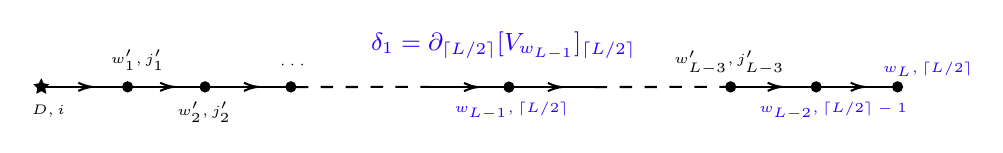
\begin{tikzpicture}[x=0.75pt,y=0.75pt,yscale=-1,xscale=1]
%uncomment if require: \path (0,149); %set diagram left start at 0, and has height of 149

%Straight Lines [id:da47312310535779345] 
\draw    (182.63,92.83) -- (224.23,92.83) ;
\draw [shift={(207.03,92.83)}, rotate = 180] [color={rgb, 255:red, 0; green, 0; blue, 0 }  ][line width=0.75]    (6.56,-1.97) .. controls (4.17,-0.84) and (1.99,-0.18) .. (0,0) .. controls (1.99,0.18) and (4.17,0.84) .. (6.56,1.97)   ;
%Straight Lines [id:da20220057529016144] 
\draw    (224.23,92.83) -- (263.43,92.83) ;
\draw [shift={(247.43,92.83)}, rotate = 180] [color={rgb, 255:red, 0; green, 0; blue, 0 }  ][line width=0.75]    (6.56,-1.97) .. controls (4.17,-0.84) and (1.99,-0.18) .. (0,0) .. controls (1.99,0.18) and (4.17,0.84) .. (6.56,1.97)   ;
%Shape: Ellipse [id:dp8548063608673344] 
\draw  [color={rgb, 255:red, 0; green, 0; blue, 0 }  ,draw opacity=1 ][fill={rgb, 255:red, 0; green, 0; blue, 0 }  ,fill opacity=1 ] (219.94,92.83) .. controls (219.94,91.62) and (220.9,90.64) .. (222.09,90.64) .. controls (223.27,90.64) and (224.23,91.62) .. (224.23,92.83) .. controls (224.23,94.04) and (223.27,95.03) .. (222.09,95.03) .. controls (220.9,95.03) and (219.94,94.04) .. (219.94,92.83) -- cycle ;
%Shape: Ellipse [id:dp3228287320589721] 
\draw  [color={rgb, 255:red, 0; green, 0; blue, 0 }  ,draw opacity=1 ][fill={rgb, 255:red, 0; green, 0; blue, 0 }  ,fill opacity=1 ] (182.63,92.83) .. controls (182.63,91.62) and (183.59,90.64) .. (184.78,90.64) .. controls (185.96,90.64) and (186.92,91.62) .. (186.92,92.83) .. controls (186.92,94.04) and (185.96,95.03) .. (184.78,95.03) .. controls (183.59,95.03) and (182.63,94.04) .. (182.63,92.83) -- cycle ;
%Shape: Ellipse [id:dp14278261604515208] 
\draw  [color={rgb, 255:red, 0; green, 0; blue, 0 }  ,draw opacity=1 ][fill={rgb, 255:red, 0; green, 0; blue, 0 }  ,fill opacity=1 ] (261.29,92.83) .. controls (261.29,91.62) and (262.25,90.64) .. (263.43,90.64) .. controls (264.62,90.64) and (265.58,91.62) .. (265.58,92.83) .. controls (265.58,94.04) and (264.62,95.03) .. (263.43,95.03) .. controls (262.25,95.03) and (261.29,94.04) .. (261.29,92.83) -- cycle ;
%Straight Lines [id:da003325442258682587] 
\draw    (475.33,92.83) -- (516.93,92.83) ;
\draw [shift={(499.73,92.83)}, rotate = 180] [color={rgb, 255:red, 0; green, 0; blue, 0 }  ][line width=0.75]    (6.56,-1.97) .. controls (4.17,-0.84) and (1.99,-0.18) .. (0,0) .. controls (1.99,0.18) and (4.17,0.84) .. (6.56,1.97)   ;
%Straight Lines [id:da4680345998514087] 
\draw    (516.53,92.83) -- (555.73,92.83) ;
\draw [shift={(539.73,92.83)}, rotate = 180] [color={rgb, 255:red, 0; green, 0; blue, 0 }  ][line width=0.75]    (6.56,-1.97) .. controls (4.17,-0.84) and (1.99,-0.18) .. (0,0) .. controls (1.99,0.18) and (4.17,0.84) .. (6.56,1.97)   ;
%Shape: Ellipse [id:dp7402103326243591] 
\draw  [color={rgb, 255:red, 0; green, 0; blue, 0 }  ,draw opacity=1 ][fill={rgb, 255:red, 0; green, 0; blue, 0 }  ,fill opacity=1 ] (514.39,92.83) .. controls (514.39,91.62) and (515.35,90.64) .. (516.53,90.64) .. controls (517.72,90.64) and (518.68,91.62) .. (518.68,92.83) .. controls (518.68,94.04) and (517.72,95.03) .. (516.53,95.03) .. controls (515.35,95.03) and (514.39,94.04) .. (514.39,92.83) -- cycle ;
%Shape: Ellipse [id:dp33457284984436353] 
\draw  [color={rgb, 255:red, 0; green, 0; blue, 0 }  ,draw opacity=1 ][fill={rgb, 255:red, 0; green, 0; blue, 0 }  ,fill opacity=1 ] (473.19,92.83) .. controls (473.19,91.62) and (474.15,90.64) .. (475.33,90.64) .. controls (476.52,90.64) and (477.48,91.62) .. (477.48,92.83) .. controls (477.48,94.04) and (476.52,95.03) .. (475.33,95.03) .. controls (474.15,95.03) and (473.19,94.04) .. (473.19,92.83) -- cycle ;
%Shape: Ellipse [id:dp15788767270693183] 
\draw  [color={rgb, 255:red, 0; green, 0; blue, 0 }  ,draw opacity=1 ][fill={rgb, 255:red, 0; green, 0; blue, 0 }  ,fill opacity=1 ] (553.59,92.83) .. controls (553.59,91.62) and (554.55,90.64) .. (555.73,90.64) .. controls (556.92,90.64) and (557.88,91.62) .. (557.88,92.83) .. controls (557.88,94.04) and (556.92,95.03) .. (555.73,95.03) .. controls (554.55,95.03) and (553.59,94.04) .. (553.59,92.83) -- cycle ;
%Straight Lines [id:da6823304743769049] 
\draw    (329.03,92.94) -- (370.63,92.94) ;
\draw [shift={(353.43,92.94)}, rotate = 180] [color={rgb, 255:red, 0; green, 0; blue, 0 }  ][line width=0.75]    (6.56,-1.97) .. controls (4.17,-0.84) and (1.99,-0.18) .. (0,0) .. controls (1.99,0.18) and (4.17,0.84) .. (6.56,1.97)   ;
%Straight Lines [id:da7777906585345375] 
\draw    (370.63,92.94) -- (409.83,92.94) ;
\draw [shift={(393.83,92.94)}, rotate = 180] [color={rgb, 255:red, 0; green, 0; blue, 0 }  ][line width=0.75]    (6.56,-1.97) .. controls (4.17,-0.84) and (1.99,-0.18) .. (0,0) .. controls (1.99,0.18) and (4.17,0.84) .. (6.56,1.97)   ;
%Shape: Ellipse [id:dp03821596864882393] 
\draw  [color={rgb, 255:red, 0; green, 0; blue, 0 }  ,draw opacity=1 ][fill={rgb, 255:red, 0; green, 0; blue, 0 }  ,fill opacity=1 ] (366.34,92.94) .. controls (366.34,91.73) and (367.3,90.75) .. (368.49,90.75) .. controls (369.67,90.75) and (370.63,91.73) .. (370.63,92.94) .. controls (370.63,94.15) and (369.67,95.14) .. (368.49,95.14) .. controls (367.3,95.14) and (366.34,94.15) .. (366.34,92.94) -- cycle ;
%Straight Lines [id:da4466392212765721] 
\draw  [dash pattern={on 4.5pt off 4.5pt}]  (409.83,92.94) -- (474.13,92.83) ;
%Straight Lines [id:da9214575197947042] 
\draw  [dash pattern={on 4.5pt off 4.5pt}]  (265.83,92.94) -- (330.13,92.83) ;
%Straight Lines [id:da024178001704609153] 
\draw    (143.18,92.83) -- (184.78,92.83) ;
\draw [shift={(167.58,92.83)}, rotate = 180] [color={rgb, 255:red, 0; green, 0; blue, 0 }  ][line width=0.75]    (6.56,-1.97) .. controls (4.17,-0.84) and (1.99,-0.18) .. (0,0) .. controls (1.99,0.18) and (4.17,0.84) .. (6.56,1.97)   ;
%Shape: Star [id:dp3258303765586473] 
\draw  [fill={rgb, 255:red, 0; green, 0; blue, 0 }  ,fill opacity=1 ] (143.18,89.81) -- (144.05,91.61) -- (145.99,91.9) -- (144.59,93.3) -- (144.92,95.28) -- (143.18,94.34) -- (141.44,95.28) -- (141.77,93.3) -- (140.37,91.9) -- (142.31,91.61) -- cycle ;

% Text Node
\draw (175.2,73.52) node [anchor=north west][inner sep=0.75pt]  [font=\tiny]  {$w'_{1} ,j'_{1}$};
% Text Node
\draw (207.2,98.52) node [anchor=north west][inner sep=0.75pt]  [font=\tiny]  {$w'_{2} ,j'_{2}$};
% Text Node
\draw (256.53,79.19) node [anchor=north west][inner sep=0.75pt]  [font=\tiny]  {$\cdots $};
% Text Node
\draw (487.67,98.86) node [anchor=north west][inner sep=0.75pt]  [font=\tiny,color={rgb, 255:red, 40; green, 0; blue, 255 }  ,opacity=1 ]  {$w_{L-2} ,\lceil L/2 \rceil - 1$};
% Text Node
\draw (547.33,79.19) node [anchor=north west][inner sep=0.75pt]  [font=\tiny,color={rgb, 255:red, 40; green, 0; blue, 255 }  ,opacity=1 ]  {$w_{L} , \lceil L/2 \rceil$};
% Text Node
\draw (446.67,73.84) node [anchor=north west][inner sep=0.75pt]  [font=\tiny]  {$w'_{L-3} ,j'_{L-3}$};
% Text Node
\draw (340.8,98.84) node [anchor=north west][inner sep=0.75pt]  [font=\tiny,color={rgb, 255:red, 40; green, 0; blue, 255 }  ,opacity=1 ]  {$w_{L-1} , \lceil L/2 \rceil$};
% Text Node
\draw (300.6,64.82) node [anchor=north west][inner sep=0.75pt]  [font=\small,color={rgb, 255:red, 40; green, 0; blue, 255 }  ,opacity=1 ]  {$ \delta_1 = \partial _{ \lceil L/2 \rceil}[ V_{w_{L-1}}]_{ \lceil L/2 \rceil}$};
% Text Node
\draw (137.13,100.24) node [anchor=north west][inner sep=0.75pt]  [font=\tiny]  {$D,i$};


\end{tikzpicture}